\documentclass[12pt]{report}

\usepackage[utf8]{inputenc}
\usepackage[french]{babel}
\usepackage[T1]{fontenc}
\usepackage{longtable}
\usepackage{graphicx}
\usepackage{verbatim} 
\usepackage{hyperref}
\usepackage{lastpage}

%-------------------------------------------------------------------------------------------------------------------------------
% Marges
\usepackage[top=2cm, bottom=2cm, left=2cm, right=2cm]{geometry}
%-------------------------------------------------------------------------------------------------------------------------------

%-------------------------------------------------------------------------------------------------------------------------------
% Entete et pied de page
\usepackage{fancyhdr} 
\fancypagestyle{plain}{%
	\fancyhf{} 
	\fancyhead{}                  
	\fancyfoot{}   
	\fancyfoot[L]{Ufwi}
	\fancyfoot[C]{\thepage \/ \pageref{LastPage}}
	\fancyfoot[R]{\today}
	\chead{Projet tuteuré – Ufwi}
	\renewcommand{\headrulewidth}{1pt}   
	\renewcommand{\footrulewidth}{1pt}      
}
\pagestyle{plain}
%-------------------------------------------------------------------------------------------------------------------------------




%-------------------------------------------------------------------------------------------------------------------------------
% Gestion de l'affichage des chapitres
\makeatletter
\renewcommand{\@chapapp}{}
\makeatother
%-------------------------------------------------------------------------------------------------------------------------------

\title{Ufwi}
\author{Maxime Robin, Cyril Pierré, Valentin Frolich, Simon Barotte}
\date{\today}

\begin{document}



%-------------------------------------------------------------------------------------------------------------------------------
% Page d'accueil
\thispagestyle{empty}
\begin{center}
Licence Professionnel ASRALL


\vspace{1cm}
Projet tuteuré.

\vspace{2,5cm}

\begin{center}
  
\includegraphics[width=10cm,height=10cm]{images/ufwi.png}
\end{center}

\vspace{1cm}
\textbf{\Huge Ufwi}


\end{center}

\vspace{4cm}

Groupe :
\begin{itemize}
  \item Cyril PIERRÉ
  \item Maxime ROBIN
  \item Valentin FROLICH
  \item Simon BARROT
\end{itemize}


%-------------------------------------------------------------------------------------------------------------------------------

\newpage

%-------------------------------------------------------------------------------------------------------------------------------
% Sommaire
\renewcommand{\contentsname}{Sommaire}
\tableofcontents
%-------------------------------------------------------------------------------------------------------------------------------

\newpage

%-------------------------------------------------------------------------------------------------------------------------------
% Content
\chapter{Introduction}
\section{Historique}
Il faut savoir que le projet Ufwi descend du projet NuFW.
La première version publique de NuFW est sortie le 01 septembre 2003.L’idée avait germée en 2001 mais ne s’était concrétisée que le 01 septembre de l’année 2003. La société croît rapidement, créant une vingtaine d'emplois en région parisienne, et acquérant une réputation dans le milieu de la sécurité informatique. En 2009, l'entreprise décide d'abandonner le pôle service pour se concentrer sur l'édition d'un pare-feu clef en main, EdenWall, couplant NuFW avec une interface d'administration performante, cette action entraina des difficulté financiere lourde a la société.
Le 18 août 2011, soit sept ans après sa création, le tribunal du commerce de Paris a prononcé la liquidation de la société, de se fait la fin du projet NuFW.\\
Cependant le projet fut reprit sous le nom de Ufwi, offrant une reprise optimale du projet en opérant un rassemblement du code, notamment éparpillé chez les clients de la société, qui évite les mois de travail nécessaires à la récupération des modifications ayant eu lieu depuis cette date.
\section{Présentation}
Ufwi est une solution de pare-feu par authentification, cela signifie qu'il effectue une authentification de chaque connexion qui le traverse. L'authentification se fait de façon transparente, en requérant les informations d’identification via l'annuaire des utilisateurs d'un réseau (LDAP ou autre). Donc avec Ufwi chaque utilisateur doit décliner son identité à chaque initialisation de conexion. Une fois que l'utilisateur est identifié, le paquet se voit filtré, selon les droits associés à l'utilisateur. Une fois que le premier paquet est accepter, les paquets suivant appartenant à la même connexion sont gérés par le système de suivi d'état (seul le paquet d'initialisation d'une connexion est authentifié). Ce principe de fonctionnement requiert la présence d'un client sur le poste utilisateur, il existe des clients compatible pour windows et GNU/Linux.
Ufwi dispose aussi d'un mode sans client, pour se faire ufwi utilise un module "ufwi-authd" (utilisé dans le cadre de notre projet).\\
Comme vu précedemment Ufwi, chaque connexion est associée à un utilisateur. Ce qui veut dire que plusieurs utilisateurs peuvent travailler sur un même poste génèrent simultanément des flux à partir d'une même adresse IP source.

\newpage
Donc Ufwi permet le filtrage par utilisateur mais peut aussi apporter d'autre fonctionalité interessantes.\newline
\begin{itemize}
    \item Ufwi permet de contribuer de manière tres pointue à la surveillance de l'activité réseau des serveurs. En regle generale dans les installations moderne on attribue des utilisateurs distinct à chaque service que fait tourner le serveur, de ce faite avec Ufwi on peut attribuer une politique réseau différente pour chaque utilisateur système.\newline
    \item Ufwi peut marquer chaque paquets d'une connexion avec les information de son utilisateur (identifiant...) ce qui permet d'appliquer une politique de qualité corespondant a chaque utilisateurs. Cela permetd onc de distribuer la bande passante en tre chaque utilisateur, ainsi attribuer une bande passante plus élevé au utilisateur qui utilise desn applications plus gourmande en terme de connexion.\newline
    \item Ufwi comprend un module de surveillance qui journalisent les événement principaux se produisant sur le réseaux en indiquant les utilisateurs à l'orgine de ses flux ( ouverture, fermeture de connexion, paquet bloqué, etc...). Ces log peuvent etre gérés au choix par Syslog, PostgreSQL ou MySQL. Ufwi conserve chaque connexion ouverte ( ou tenté) meme si l'utilisateur en question a changé d'adresse IP ou de machine.\newline
    \item Ufwi permet d'identifier les utilisateurs des aplications réseau grace a une authentification unique (Single sign on). Grace au systeme de journalisation Sql une table de connexion est maintenu en temps reel.  
%-------------------------------------------------------------------------------------------------------------------------------
\chapter{Liste des solutions de pare-feu par identification}
Les pare-feu par identification les plus connus : 
  \begin{itemize}
    \item AuthPF : Fonctionne sous OpenBSD et qui se repose sur SSH pour l'identification des utilisateurs : http://www.openbsd.org/faq/pf/authpf.html
    \item NuFW : projet ayant donné naissance à UFWI suite à la liquiditation de l'éditeur "EdenWall Technologies"
    \item Cyberoam : pare-feu entièrement basé sur l'identification, en utilisant une corrélation entre adresse MAC et utilisateur : http://www.cyberoam.com/fr/firewall.html
    \item CheckPoint (NAC Blade) : utilisation des règles de filtrage en fonction d'une authentifcation basée sur Kerberos, l'identité de son poste et du niveau de sécurité du poste ( mise à jour de sécurité / antivirus ) : http://www.cyberoam.com/fr/firewall.html
  \end{itemize}
\newligne
Ci-dessous un tableau comparatif des different avantage et inconvénient des differentes solution de pare-feu par authentification: \\
\begin{tabular}{|p{3cm}|p{5cm}|p{5cm}|}
  \hline
  Solution parefeu & Avantage & Inconvégnient\\
  \hline
	Ufwi &
 	\begin{itemize}
		\item Projet devenu libre.
		\item Appliquer des règles horaires strictes.
		\item  composé de deux démons qui peuvent être mis en place sur des systèmes différents et le démon principal est massivement multithreadé.
		\item Contrôle d’accès sont réalisées grâce à des greffons (des modules system, ldap, dbm, plaintext).
		\item Journalisation de l’activité des utilisateurs peut être faite par syslog, mysql, postgresql.
		\item Multi plate-forme.
		\item Géneration des acl grace a un module (nuaclgen)
	\end{itemize}&
	\begin{itemize}
		\item Tres peu de documenation voir aucune (obligé de cf. à nufw).
		\item Nécessite une partie cliente spécifique sur les postes clients.
		\item Payante sous windows (NuWinC).
		\item Projet peu soutenu (temps de reponse 20-30 jours).
	\end{itemize} \\
  \hline
	AuthPF&
	\begin{itemize}
		\item règles par système et/ou par utilisateur.
		\item Connection via SSH.
		\item chaque utilisateur peut disposer de ses propres règles, présentes dans HOME/.authpf/authpf .rules.
		\item Simple a metre en place.
		\item  C'est un Firewall de type filtre de paquet (Couches réseau et transport).
		\item Documentation et suport en français et assez simple.
	\end{itemize}&
	\begin{itemize}
		\item l'utilisateur se déconnecte, le pare-feu lui retire les règles ajoutées.
		\item quelqu'un d'autre peut toujours spoofer cette IP et passer.
		\item Necessite la creation d'un home pour chaque utilisateur.
		\item Necessite Openbsd et des conaissance PF.
	\end{itemize} \\
  \hline 
	Cyberoam&
	\begin{itemize}
		\item N
		\item A 
	\end{itemize}&
	\begin{itemize}
		\item N
		\item A
	\end{itemize} \\
  \hline 
	CheckPoint&
	\begin{itemize}
		\item N
		\item A
	\end{itemize}&
	\begin{itemize}
		\item N
		\item A
	\end{itemize} \\
\end{tabular} 
%-------------------------------------------------------------------------------------------------------------------------------
\chapter{Externalisation des logs dans une BD MySQL}
\underline{Configuration du serveur BD}

Installation des paquets :

apt-get install apache2 php5 mysql-server nulog

\underline{Configuration de la passerelle :}

Configuration IP :

ifconfig eth0 192.168.1.137/24
ifconfig eth1 172.20.8.1/24

Installation des paquets :

apt-get install ulogd ulogd-mysql

Correction d'un bug : ajout d’une ligne dans le script de démarrage qui va charger un module

nano /etc/init.d/ulogd
export LD_PRELOAD=/usr/lib/libmysqlclient.so.16

Configuration de ulogd : modification de son fichier de configuration

nano /etc/ulogd.conf

Décommenter la ligne 46 (pour charger un module supplémentaire)

Renseigner les informations de connexion à la base de données :

paragraphe « [MYSQL] » ligne 59 :
table=’’ulog’’
pass=’’passulog’’
user=’’ulog’’
db=’’ulog’’
host=’’172.20.8.2’’

Configuration du serveur de BD:

Configuration IP :

ifconfig eth0 172.20.8.2/24

Lister tous les fichiers installés à l’installation de nulog :

dpkg –L nulog | more

Ouvrir le fichier suvant (démarche à suivre pour creer les tables de la base de données)

nano /usr/share/doc/nulog/README.Debian

Connexion à la base de données et création de l’utilisateur (les deux programmes vont se connecter avec ce compte):

mysql –u root –p
create database ulog;
create user 'ulog'@'\%' identified by 'passulog' ;
grant all privileges on ulog.* to ulog;
exit

Commandes de création de la base :

cd /usr/share/doc/nulog/scripts
gunzip ipv4.sql.gz
cat ipv4.sql | mysql –uulog –p ulog

Modification du fichier de configuration de mysql

nano /etc/mysql//my.cnf
ligne 47

Il faut qu’il écoute sur l’interface 172.20.8.2

bind address= ‘’172.20.8.2’’

Renommer les fichiers de configuration :

cd /etc/nulog
cp default. core.conf core.conf
cp default.nulog.conf nulog.conf
cp default.wrapper.conf wrapper.conf

Renseigner les informations de connexion à la base de données :

nano core.conf
host=localhost
db=ulog
user=ulog
password=passulog
table=ulog

Prise en compte des changements : redémarrage de services
Sur la passerelle :

/etc/init.d/ulogd restart

Sur le serveur :

/etc/init.d/ulogd restart


On choisit ce que l’on veut loguer avec iptables

%-------------------------------------------------------------------------------------------------------------------------------
\chapter{Fonctionnement d'ufwi}
\section{Algorithme}

\begin{enumerate}
  \item Au démarrage de sa session de travail, l’utilisateur lance un client sur son poste de travail. Le client ouvre un tunnel crypté par TLS vers le serveur nuauth qui réalise l’authentification de l’utilisateur pour ce tunnel au regard d’un annuaire référent. Ce tunnel est ensuite conservé pendant toute la durée des opérations et l’ensemble des échanges entre nuauth et le client se fait ensuite par son intermédiaire.
  \\
  \item Supposons maintenant que l’utilisateur ouvre une connexion vers un serveur, par exemple une connexion web à destination du serveur d’application. Il utilise alors son navigateur favori qui envoie un paquet à destination du serveur. Le paquet envoyé est un paquet TCP standard avec notamment comme caractéristiques port destination 80 (web) et bit SYN positionné (ouverture de connexion).
  \\
  \item Le pare-feu (Netfilter) envoie ce paquet au démon nufw (au moyen de la décision QUEUE ou NFQUEUE) : contrairement à un pare-feu " classique ", Netfilter ne prend pas de décision à propos de cette connexion.
  \\
  \item Le démon nufw se contente de relayer le paquet reçu vers le serveur d’authentification, qui a autorité sur les décisions.
  \\
  \item Le démon nuauth analyse le paquet reçu (et en particulier l’adresse IP source) et envoie une demande de mise à jour à tous les clients connectés (par l’étape 1) depuis cette adresse pour qu’ils authentifient les connexions en attente. Cette demande est envoyée au travers du (ou des) canal (canaux) crypté(s) ouvert(s) à l’étape 1.
  \\
  \item Le client qui a ouvert notre connexion " témoin " stipule à nuauth qu’il l’a fait, en précisant tous les paramètres IP (IP et port destination, port source, etc.). À ce stade, le serveur nuauth connaît, de manière sûre, l’identité de l’utilisateur à la source de notre connexion.
  \\
  \item nuauth réalise une requête sur la base des ACL, pour vérifier si l’utilisateur dispose des droits pour établir cette connexion. nuauth obtient ainsi une décision.
  \\
  \item (En option) nuauth journalise toutes les informations relatives à cette connexion dans une base SQL, avec bien sûr l’identité de l’utilisateur.
  \\
  \item nuauth envoie la décision obtenue en 7 à nufw, qui la relaie à son tour à Netfilter. La décision associée à notre utilisateur est alors appliquée par Netfilter.
  \\
  \item S’il est autorisé, le paquet poursuit sa route.
  \\
  \item (En option) Si le serveur (Apache, par exemple) désire connaître l’identité de l’utilisateur, au lieu de la lui demander directement, il peut réaliser une simple requête SQL SELECT pour récupérer l’identifiant de l’utilisateur en partant de marqueurs uniques de la connexion (la socket source, pour les connaisseurs). L’utilisateur est ainsi authentifié de manière transparente, et sans pouvoir tricher, sur le serveur : il s’agit d’une solution de Single Sign On (authentification unique) très simple, très sûre, et indépendante du protocole.
  \\
  \item Le reste du flux est géré par le suivi de connexion (Stateful inspection) de Netfilter : les paquets ne repassent pas par les démons nufw/nuauth.
\end{enumerate}
\begin{center}
  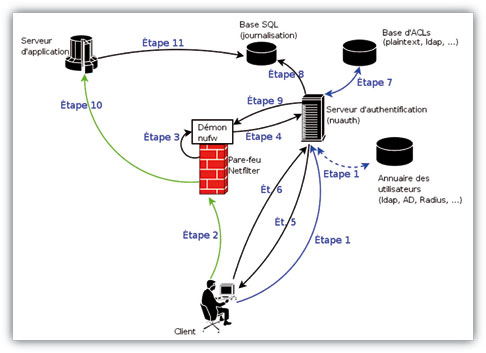
\includegraphics[width=12cm,height=10cm]{images/algo.jpg}
\end{center}

%-------------------------------------------------------------------------------------------------------------------------------
\chapter{Daemon ufwi-authd}
\section{Introduction}

Nuauth command est une interface qui permet de contrôler des fonctions importantes du daemon authd, 
comme l'obtention de la liste des utilisateurs connectés par exemple.
Chaque fois qu'un client envoie un paquet(1) pour commencer une connexion à travers la 
passerelle, la station cliente envoie un paquet(2) d'identification au daemon authd. Le 
pare-feu de la passerelle met en file d'attente le paquet et envoie directement des 
informations au daemon authd.

Le travail du daemon va être d'analyser les deux paquets (1) et (2) et de vérifier si 
le client à le droit d'initialiser la connexion qu'il demande.
Si ufwi-authd indique que le paquet(1) est autorisé alors la connexion est initialisé,
sinon la connexion est annulé. Ufwi-authd peut aussi utiliser un serveur LDAP pour la
définition des utilisateurs et groupes.

Ci-dessous le un schéma montrant le processus d'authentification utilisé par NuFW, resté inchangé avec UFWI:

\begin{center}
  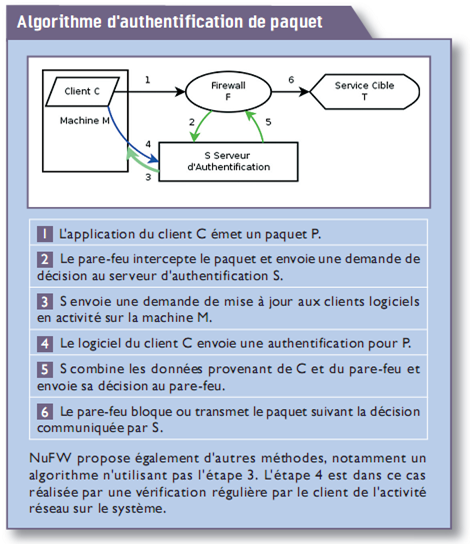
\includegraphics[width=8cm,height=10cm]{images/auth.png}
\end{center}

\section{Intallation}

Pré-requis :

Script autogen.sh :
    \begin{itemize}
      \item version automake1.7
    \end{itemize}
Compilation Nufw :
  \begin{itemize}
    \item GNU libtool
    \item GNU make
    \item libpam-dev
    \item glib 2.4+
    \item libipq (iptables-dev pour debian) ou libnetfilter queue
    \item libldap
    \item libsasl2
    \item libgnutls
    \item libgcrypt
  \end{itemize}

Noyau:

Il est recommandé d'utiliser un noyau récent afin de bénificer de toutes les dernières nouveautés implémenter dans ce dernier.
Une version de noyau supèrieur à 2.6.18 est un bon choix. Le patch dump-connection-mark.diff ( disponible dans patches/ ) 
peut être appliqué au noyau afin d'améliorer les perfomances de ce dernier lorsque nous utiliserons le log de session.

Compilation:

La compilation du daemon est relativement simple, elle se déroule en quatre étapes:
  \begin{itemize}
   \item Lancement du script ./autogen.sh
   \item Exécution de ./configure
   \item make
   \item Et pour finir make install
  \end{itemize}
Lors de la première installation, il faut penser à copier le ficheir de configuration avec la commande suivante:

cp ./conf/nuauth.conf /usr/local/etc/nuauth.conf

\section{Quelques commandes liées au daemon}

Commandes principales:
\begin{itemize}
  \item quit: déconnexion
  \item refresh cache: rafraichit tous les caches
  \item reload: recharge la configuration du daemon d'authentification 
\end{itemize}
Information:
\begin{itemize}
  \item help: affiche la liste des commandes utilisables
  \item version: affiche la version du daemon
  \item uptime: affiche depuis combien de temp tourne le daemon 
\end{itemize}
Gestion des utilisateurs:
\begin{itemize}
  \item users: affiche els utilisateurs connectés
  \item disconnect all: déconnecte tous les utilisateurs
  \item disconnect ID: déconnecte un utilisateur grâce à son identifiant (ID) 
\end{itemize}

\section{Fichier de configuration}

Le fichier authd.conf est le fichier principal de configuration pour le
daemon ufwi-authd. C'est dans ce fichier que seront indiqué l'adresse du daemon ufwi-filterd 
par exemple ou encore le niveau de debug, le nombre de connexion qu'un utilsateur peut lancer.
Dans ce fichier seront aussi renseigné les différents paramètres qui guide le comportement du 
daemon, mais aussi les paramètres système, et pour finir les chemins absolus des autres fichiers
de configuration.

Il existe aussi d'autres fichiers de configurations liés à ufwi-authd:
\begin{itemize}
  \item modules/nuauth-tls.conf qui contiendra les paramètres TLS
  \item modules/nuauth-krb5.conf configuration authentification Kerberos 5
  \item modules/nuauth-ldap.conf authentification ldap
  \item modules/nuauth-mysql.conf configuration de la base de donnée pour les logs utilisateurs (mysql)
  \item modules/nuauth-pgsql.conf configuration de la base de donnée pour les logs utilisateurs (postgres) 
\end{itemize}
 
\section{Installation des certificats}

Le daemon d'authentification et le client utilise des certificats afin de comuniquer ensemble. Lors de l'installation de la
suite ufwi des certificats sont installés par défaut dans le répertoire /certs. On peut utiliser ces certificats par défaut 
pour procéder à des tests mais il n'est pas conseillé de les utiliser pour un utilisation pro de la suite ufwi. Dans cette 
section nous allons voir comment générer ces certificats.

Génére notre propre Authorité de Certification:

\textit{mkdir private}

\textit{chmod 700 private}

\textit{openssl req -new -x509 -keyout private/CAkey.pem -out private/CAcert.pem}

Génére les clefs privées pour le client et le daemon d'authentification:

\textit{openssl genrsa -out private/nufw-key.pem}

\textit{openssl genrsa -out private/nuauth-key.pem}

Génére les demandes de certificats pour le client et le daemon:

\textit{openssl req -new -key private/nufw-key.pem -out nufw.csr}

\textit{openssl req -new -key private/nuauth-key.pem -out nuauth.csr}

Signe les demandes de certificats grâce à l’AC:

\textit{openssl x509 -req -days 365 -in nufw.csr -CA private/CAcert.pem -CAkey private/CAkey.pem -CAcreateserial -out nufw-cert.pem}

\textit{openssl x509 -req -days 365 -in nuauth.csr -CA private/CAcert.pem -CAkey private/CAkey.pem -CAcreateserial -out nuauth-cert.pem}
\\
Enfin on déplace les certificats dans le bon répertoire:

\textit{cp private/nufw-key.pem /etc/nufw/}

\textit{cp nufw-cert.pem /etc/nufw/}

\textit{cp private/nuauth-key.pem /etc/nufw/}

\textit{cp nuauth-cert.pem /etc/nufw/}

\section{Configuration basique du daemon}

Lors de l'installation de la suite ufwi un fichier de configuration de base est fournie nuauth.conf, qui est disponible 
dans le répertoire conf.
Ce fichier est remplie de plusieurs directives, les deux plus importantes directives de configuration sont : 
nuauth client listen addr : qui définit l’adresse à laquelle le daemon va attendre les requètes des clients 
nuauth nufw listen addr : qui définit l’adresse à laquelle le daemon va attendre les requètes de nufw. 
La liste des machines autorisées à se connecter au serveur d'authentifcation constitue la variable nufw gw addr.

Ensuite, on doit choisir le module d’authentification et de vérification des ACL. Les modules suivants sont disponibles :
\begin{itemize}
 \item libldap : les informations utilisateur sont stockées dans un annuaire LDAP
 \item dbm : les informations utilisateur sont stockées dans une base gdbm
 \item plaintext : les informations utilisateur sont stockées dans un fichier texte
 \item system : l’authentification s’adosse à PAM et utilise les groupes existants dans le système. Ceci procure un 
moyen pratique d’utiliser nss et/ou pam-modules
\end{itemize}

Le module d’authentification est paramétrable via l’option nuauth user check module dont la valeur par défaut est
libsystem (si non défini dans le fichier de configuration). D’autre paramètres concernant la vérification
des ACL doivent être précisés si on choisit une des deux authentification suivante :
\begin{itemize}
 \item libldap
 \item plaintext
\end{itemize}
Tout ceci en définissant la variable nuauth acl check module.

%-------------------------------------------------------------------------------------------------------------------------------
\chapter{Daemon ufwi-filterd}
\section{Introduction}

	Le daemon ufwi-filterd (ancienement appelé nufw) n'est d'autre qu'un pare-feu basé sur NFQUEUE netfilter. Il permet d'écrire des règles de filtrage basées sur l'identité des utilisateurs, en plus des critères de réseau classiques. L'authentification effectue de façon transparente en requérant les informations d’identification de l’utilisateur avantqu’une quelconque décision de filtrage ne soit prise. En pratique, cela signifie que les politiques defiltrage peuvent intégrer l’annuaire utilisateur, et amène cette notion d’ID utilisateur au niveau de la couche IP.\\
Ufwi-filterd est capable de:
\begin{itemize}
  \item Filtrer le trafic en fonction du système d’exploitation et des applications utilisées par les utilisateurs
     distants.
  \item marquer chaque paquet d'une connexion avec l'identifiant de son utilisateur et donc d'appliquer une politique de qualité de service spécifique à chaque utilisateur. 
  \item contribue de manière très pointue à la surveillance de l'activité réseau des serveurs.
  \item dispose de modules de surveillance qui journalisent les événements principaux de l'activité du réseau en indiquant quels sont les utilisateurs à l'origine des flux.
\end{itemize}
\section{Intallation}
Une installation typique de la suite logicielle NuFW comporte 2 démons : nufw (ufwi-filterd) et nuauth (ufwi-authd) et autant de clients que nécessaire.\\
Pré-requis :
\begin{itemize}
  \item automake1.7 pour executer autogen.sh
  \item GNU libtool
  \item GNU make
\end{itemize}
Pré-requis pour la compilation et l'excution de ufwi-filterd :
\begin{itemize}
  \item ufwi-base
  \item ufwi-confparser
  \item ufwi-ssl
\end{itemize}
Il est recommandé d'utiliser un noyau récent afin de béneficer de toutes les dernières nou-
veautés implémenter dans ce dernier. Une version de noyau supèrieur à 2.6.18 est un bon choix.
\newpage
\section{Compilation}
La compilation de ufwi-filterd est relativement simple elle se resume a utiliser les commandes suivantes :
\begin{itemize}
  \item ./autogen.sh
  \item ./configure
  \item make
  \item makeinstall
\end{itemize}
Lors de la première installation, il ne faut pas oublier de copier le fichier de configuration "make install-conf" afin de chercher les changements entre votre fichier de conf actuelle et le nouveau.\\
Un fichier INSTALL avec toutes les instructions a suivre est fournie dans le dossier de ufwi-filerd disponible a partir de se lien http://ufwi.org/projects/ufwi-filterd/ repository .
\section{Commandes}
Tout dabord, vous devez executer en root ufwi-filterd.
ufwi-filterd -h vous donnera un message d'aide pour l'utilisation de ufwi-filterd.
\section{Fichier de configuration}
Le fichier de configuration de ufwi-filterd se nome tout simplement "filterd.conf". On poura le trouver dans /etc/ufwi-filterd/.
Dans se fichier on trouvera l'adresse ou le nom du serveur d'authentification nuauth (par defaut 127.0.0.1), on trouvera aussi les chemin absolut des fichiers :
\begin{itemize}
  \item /etc/ufwi-filterd/key.pem (clé privé du serveur)
  \item /etc/ufwi-filterd/cert.pem (certificat du serveur)
  \item /etc/ufwi-filterd/cacert.pem
  \item /etc/ufwi-filterd/crl.pem (liste de révocation de certificat serveur)
\end{itemize}

%-------------------------------------------------------------------------------------------------------------------------------
\chapter{Daemon ufwi-rcpd}
\section{Introduction}
Le module ufwi-rcpd (anciènnement appelé NuCentral) est le module qui gère les autres deamons.

\section{Installation}
\subsection{Pré-requis}
Avant de lancer l'installation du module, certains pré-requis sont nécéssaires :
\begin{itemize}
  \item Python 2.5
  \item Twisted web
  \item M2Crypto
  \item Jinja
  \item Subversion (svnadmin program)
  \item sudo
  \item pysvn
  \item pytz
\end{itemize}
Debian: \begin{verbatim}apt-get install python-twisted-web python-svn 
    python-m2crypto sudo python-jinja subversion python-tz\end{verbatim}
\newline

Pour l'installation de ufwi-rpcd:
\begin{itemize}
  \item (GNU) make
  \item sqlite3
\end{itemize}
Sous Debian: \begin{verbatim}apt-get install make sqlite3\end{verbatim}
\newline

Paquets optionnels :
Pour compiler les fichiers de .ts à .qm et mettre à jours les transmissions :
\begin{itemize}
  \item lrelease4: Qt development tools
  \item pylupdate4, lrelease-qt4: Python Qt development tools
\end{itemize}
Sous Debian: \begin{verbatim}apt-get install libqt4-dev pyqt4-dev-tools\end{verbatim}
\newline

Autres :
\begin{itemize}
  \item python-twisted-snmp : pour le module SNMP.
  \item gnutls-bin : le programme certtool l'utilise pour générer les certificats ssl.
  \item py.test (Sous Debian, python-codespeak-lib) : utilisé pour les tests.
  \item libconfig-inifiles-perl : pour tools/ufwi\_rpcd\_enmod.
  \item IPy (python-ipy) : pour les tests.
\end{itemize}

\section{Utilisation}
Une fois démarrer, on peut accèder au fonction plus particuliaire de ufwi-rpcd (nucentral).
\subsection{Démarrage}
\subsubsection{Lancement en mode deamon}
Pour lancer ufwi-rpcd en mode deamon il suffit d'exécuter une commande en root:
\begin{verbatim}
twistd -y /usr/sbin/ufwi-rpcd.tac --pidfile=/var/run/ufwi-rpcd.pid 
    -l /var/log/ufwi-rpcd-twisted.log
\end{verbatim}
   
Pour arrèter ufwi-rpcd en mode deamon (en root):
\begin{verbatim}kill \$(cat /var/run/ufwi-rpcd.pid)\end{verbatim}
   
\subsubsection{Lancement en mode "premier plan"}
Pour facilité le développement, on peut également lancer ufwi-rpcd en premier plan:
\begin{verbatim}twistd -n -y /usr/sbin/ufwi-rpcd.tac -l /var/log/ufwi-rpcd-twisted.log\end{verbatim}
Pour arréter le processus : CTRL+c.

\subsection{ufwi\_rpcd\_client (nucentral\_client)}
\subsubsection{Le client}
Pour lancer le client d'ufwi\_rpcd en HTTP (tcp/8080):
\begin{verbatim}ufwi_rpcd_client --host 127.0.0.1 --cleartext -u admin -p admin\end{verbatim}
Par défaut, ufwi\_rpcd\_client utilise HTTPS (tcp/8443):
\begin{verbatim}ufwi_rpcd_client --host 127.0.0.1 -u admin -p admin\end{verbatim}
Une fois connecté sur le client, le prompt devient: 
\begin{verbatim}nucentral>\end{verbatim}

\subsubsection{Le menu}
Une fois lancer, on peut accèder aux différentes fonctions d'ufwi-rpcd:
\begin{itemize}
  \item \begin{verbatim}call('component', 'service', ...)\end{verbatim}
  Apelle un service d'NuCentral
  \item \begin{verbatim}authenticate('login', 'password')\end{verbatim}
  Authentification ou mise à jour d'un groupe ou d'un utilisateur.
  \item \begin{verbatim}components()\end{verbatim}
  Affiche la liste des différents composants.
  \item \begin{verbatim}services('component')\end{verbatim}
  Affiche la liste des services d'un composant.
  \item \begin{verbatim}proxy('component')\end{verbatim}
  Créé un composant pour le proxy qui pourra être utilisé avec component.service().
  \item \begin{verbatim}nucentralStatus()\end{verbatim}
  Afficher l'état du serveur et la session d'informations.
  \item \begin{verbatim}help('component')\end{verbatim}
  Utilisation d'un composant.
  \item \begin{verbatim}help('component', 'service')\end{verbatim}
  Utilisation d'un service d'un composant.
  \item \begin{verbatim}help(proxy)\end{verbatim}
  Utilisation du proxy.
  \item \begin{verbatim}exit()\end{verbatim}
  Quitter.
  \item \begin{verbatim}pyhelp(object)\end{verbatim}
  Aide Python pour l'objet spécifié.
  
\end{itemize}
\\
\\
Différents composants sont disonibles :
\begin{verbatim}
CORE, access, acl, audit, auth_cert, bind, config, contact, hostname, hosts, 
httpout, localfw, lock, logger, network, ntp, nuauth, nuauth_command, nuconf, 
nuface, nulog, nupki, nurestore, reporting, resolv, session, status, streaming, 
system, system_info, tools, update, users_config, versionning
\end{verbatim}


%---------------------------------------------------------------------------------------------------------------------------------
\chapter{Avencement du projet à mis parcours}
Ce qui a été fait :
\begin{itemize}
  \item Ufwi est installé et fonctionnel.
  \item La première partie du projet est terminer. Il reste les tests de fonctionnement à faire
\end{itemize}


Ce qui reste a faire :
\begin{itemize}
  \item Recherche des limites et des failles du logiciel
  \item Comment gérer l'élévation de privilèges (root se connect en ssh sur un non-root, que se passe t-il ?)
  \item Mettre en lumière les durées de vie des autorisations données.
  \item Comment s'assurer que l'utilisateur est encore présent ?
  \item Ufwi aide t-il pour l'authentification des utilisateurs nomades connu (commercial) ou non (intervenant exterieur) ?
\end{itemize}
  

%---------------------------------------------------------------------------------------------------------------------------------
\chapter{Difficulté rencontré et avis personnel}
%---------------------------------------------------------------------------------------------------------------------------------
\end{document}
